
\section{Teknologibeskrivelse}
Aktivitetsarmbånd bliver i stigende grad mere udbredt. Ifølge IDC er der sket en stigning i salget af aktivitetsarmbånd fra 11,8 millioner enheder i første kvartal af 2015 til 19,7 millioner i første kvartal af 2016 \citep{IDC2016}.

Det har ikke været muligt at finde statistisk data vedrørende udbredelsen af Fitbit Flex armbåndet, dog ses at Fitbit udgør stor andel af markedet for aktivitetsarmbånd, og at der fra første kvartal i 2015 til første kvartal i 2016 er sket en stigning i salget på 1 million enheder \citep{IDC2016}.  
Fitit Felx armbåndet, som det vil båret af brugeren, ses af \autoref{fig:fitbitflexarmbånd}. 

\begin{figure}[H]
	\centering
	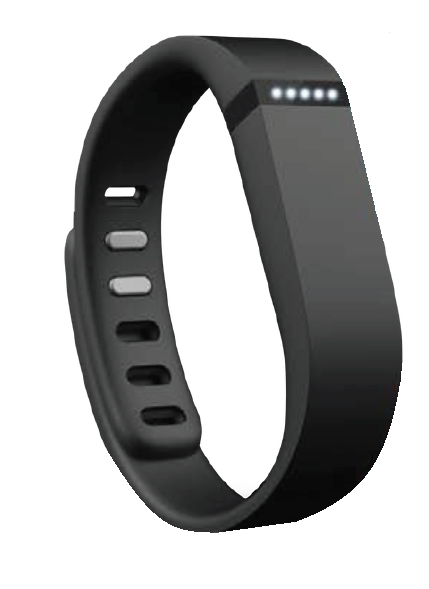
\includegraphics[width=0.35\textwidth]{figures/fitbitflex}
	\caption{Fitbit flex armbånd \citep{fitbitflex}.}
	\label{fig:fitbitflexarmbånd}
\end{figure}

Overordnet består et Fitbit Flex aktivitetsarmbånd af en flex tracker, oplader kabel, trådløs synkroniserings dongle og armbånd til flex tracker \citep{fitbitflex}. Disse kan ligeledes ses af \autoref{fig:fitbitflexindhold}. 

\begin{figure}[H]
	\centering
	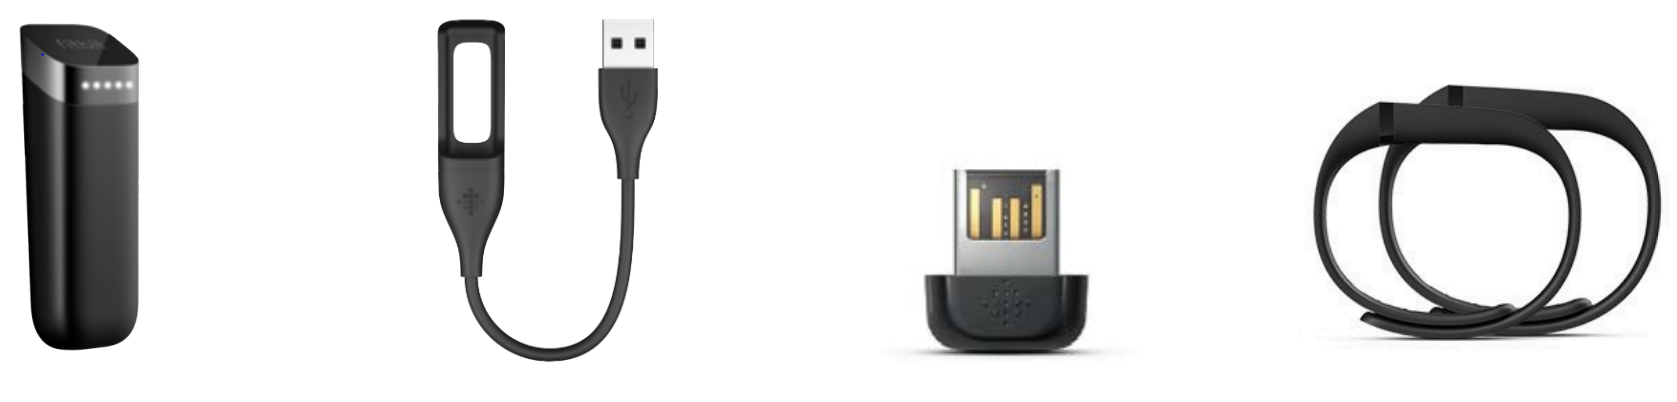
\includegraphics[width=0.6\textwidth]{figures/fitbitflexindhold}
	\caption{Fra venstre mod højre ses flex tracker, oplader kabel, trådløs synkroniserings dongle, armbånd \citep{fitbitflex}.}
	\label{fig:fitbitflexindhold}
\end{figure}

Fitbit Flex er i stand til at måle antal skridt, forbrændte kalorier, afstand dækket, minutter brugeren er aktiv og længden samt kvalitet af søvn. 
For at brugeren kan se den registrerede aktivitet, som er blevet opsamlet af armbåndet, skal dette synkroniseres med en kompatibel enhed, da armbåndet kun besidder et display bestående af fem LED'er. 
Synkronisering foregår trådløst, ved brug af bluetooth low energy og kan foregå mellem forskellige enheder som for eksempel smartphone og computer. 
Synkronisering mellem flex tracker og computer kræver dog anvendelse af den trådløs synkroniserings dongle, der ses af \autoref{fig:fitbitflexindhold}.
Forudsætninger for, at data kan synkroniseres er, at en kompatibel enhed har den korrekte applikation installeret, hvor synkroniseringen ellers sker automatisk idet applikationen åbnes.  
Yderligere skal der oprettes en brugerkonto på www.fitbit.com, hvor brugeren oplyser personlig info: køn, alder, højde og vægt. Dette er nødvendigt i forhold til optimering af dataopsamling og estimering af forbrændte kalorier.  
Gennem applikationen visualiseres den registrerede aktivitet, hvor brugeren har mulighed for at se data fra starttidspunktet for anvendelsen af armbåndet. Data kan også observeres via  Fitbits hjemmeside, hvor det er muligt at logge ind via brugerkontoen. 
Således ville alle i besiddelse af brugerkontoen have adgang til den synkroniserede data, uden fysisk at havde hverken bruger eller armbånd til rådighed. 
Til den daglige aktivitet har brugeren mulighed for at sætte bestemte mål til den fysiske aktivitet. Alt efter hvilke mål brugeren sætter for sig selv, kan progressionen ses ud fra de fem LED'er på armbåndet, ved at brugeren trykker to gange på armbåndet.   
Når et af brugerens mål gennemføres, visualiseres dette ved at de 5 LED'er blinker og at armbåndet vibrerer. 
Fitbit Flex armbåndet er ikke i stand til at visualisere batteriniveauet for armbåndet, dette kan dog ses ved brug af applikationen. 
Hukommelsen i flex trackeren tillader detaljeret data at blive lagret i perioder op til 7 dage og består af minut til minut målinger.  
Yderligere lagres summeringer af daglig aktivitet i op til 30 dage. 
Ved jævnlig synkronisering er det muligt for brugeren at bevare detaljeret data, da informationen tilknyttes brugerkontoen. 
Fitbit anbefaler én daglig synkronisering, dog er det ikke en nødvendighed \citep{fitbitflex}. 

\subsection{Hardware}
Fitbit flex trackeren har forskellige hardware elementer, hvorfra trackeren signalere, og detektere fysisk aktivitet. Hardwaren i trackeren udgøres af et display, sensor, motorer og batteri.
 
\textbf{Display:} 
Flex trackeren er udstyret med fem LED'er, der ved forskellige operationstilstande signalerer til brugeren. 
LED'erne fungerer for eksempel, som indikator for progressionen i forhold til det brugerdefinerede fysiske mål for dagen. Hertil vil hver LED repræsentere en procentvis progressionen i intervaller af $20 \%$. Eksempelvis hvis brugeren har opfyldt $73 \%$ af det fysisk mål, vil de første tre LED'er lyse og den fjerde vil blinke. Dette indikerer, at brugeren har nået $60 \%$ af målet, og at brugeren nu befinder sig mellem $60 \%$ og $80 \%$. 
Det samme gør sig gældende når flex trackeren sættes til opladning. Her indikerer LED'erne, hvor langt armbåndet er fra fuld opladning, som signaleres ved at alle fem LED'er lyser. 
I tilfælde af synkroniseringsfejl vil dette også fremgå af LED'erne. Her vil armbåndet lyse med et mønster, skiftevis mellem at have ingen eller alle LED'er tændt. 
Ved manuel aktivering og de-aktivering af sleep mode, vil LED'erne indikere dette gennem forskellige indikationsmønstre.

\textbf{Sensor:} 
Flex trackeren registrer den fysiske aktivitet ved anvendelse af et MEMS 3-akses accelerometer, hvilket er den eneste sensor, som er implementeret i armbåndet. Ud fra algoritmer analyseres bevægelsesmønstre, hvorved der kan oplyses hvor mange skridt der er foretaget under løb eller gang, den tilbagelagte afstand, med mere. 

\textbf{Motorer:}
Flex trackeren er yderligere udstyret med en vibrationsmotor, der aktiveres under forskellige funktioner når armbåndet anvendes. Disse fungerer i sammenspil med displayet, som et kommunikationsredskab for brugeren. Vibration aktiveres ved anvendelse af alarm funktion og ved aktivering eller de-aktivering af sleep mode, samt når det daglige fysiske mål nåes. 
 
\textbf{Batteri:} 
Fitbit Flex indeholder et genopladeligt batteri, der lades ved brug af det medfølgende kabel. Dette ses af \autoref{fig:fitbitflexindhold}. Kablet tilsluttes en computer og opladningen begynder, hvis computeren er tændt. 
Levetiden på batteriet er op til 5 dage, dog kan mindre forventes ved omstændigt brug.


\subsection{Software}
Applikationen er brugerfladen hvorfor den synkroniserede data formidles til brugeren. Her oplyses skridt, forbrændte kalorier med mere. 
Alt efter brugerens engagement, kan der også udfyldes informationer omkring indtaget kost ved brug af applikationen. Brugeren kan ud fra dette få et estimat af hvor mange kalorier der indtages, hvortil dette kan sammenlignes med antal kalorier forbrændt. Anvendelsen af denne kost-log er dog ikke en nødvendighed for anvendelsen af armbåndet eller applikationen, dog kunne dette give en praktiserende læge indblik i om patienten overholder anbefalingerne for hypertensive patienter, både i forhold til kostvaner, samt fysisk aktivitet.  

\begin{figure}[H]
	\centering
	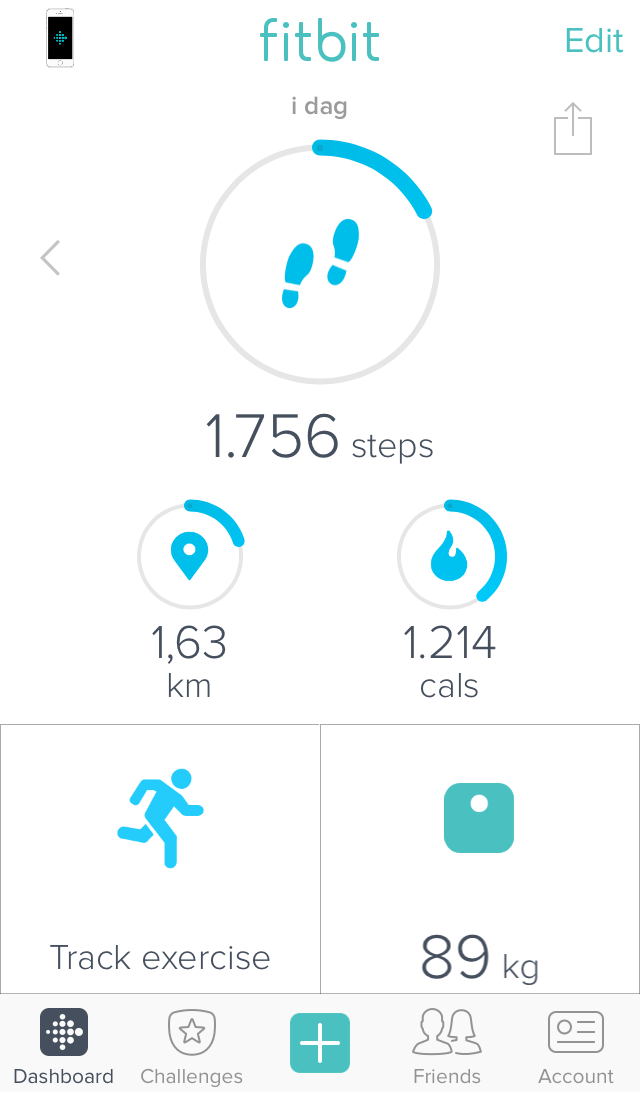
\includegraphics[width=0.45\textwidth]{figures/burgerfladeoversigt}
	\caption{Ooverordnet oversigt af fysisk aktivitet, der vises idet applikationen åbnes. Her vises antal skridt taget, afstand rejst, kalorier forbrændt med mere.}
	\label{fig:brugerfladeoversigt}
\end{figure}

Af \autoref{fig:brugerfladeoversigt} ses oversigt over den registrerede aktivitet som er målt gennem armbåndet. Her ses skridt taget, afstand rejst og kalorier forbrændt. Af oversigten ses også hvor langt brugeren er fra at opfylde de forskellige aktivitetsmål, og er repræsenteret af den blå cirkel omkring de forskellige angivelser. 
Af bunden ses fire forskellige oversigter, hvor der fra venstre mod højre ses dashboard, challenges, friends og account. Plus tegnet i midten fungerer som en genvej til forskellige funktioner under de fire oversigte. 
\textbf{Dashboardet} er den overordnede oversigt, som oplyser det førnævnte (ydet aktivitet). 
\textbf{Challenges} viser en oversigt over tilvalgte aktivitetsudfordringer, hvor brugeren har mulighed for at opstille udfordringer med venner samt andre brugere af applikationen. 
\textbf{Friends} giver brugeren et overblik og venner der er tilføjet til applikationen. 
\textbf{Account} viser overblik over hvilken bruger der er logget ind, og hvilken fitibt enhed der er tilsluttet applikationen. Yderligere kan der fortages ændringer af profil og mål for daglig fysisk aktivitet. 

En detaljeret oversigt over ydet aktivitet kan ses under den overordnede oversigt, ved at tykke på de specifikke målinger. Ved at trykke på steps ses eksemplet der fremgår af \autoref{fig:brugerfladesteps}.  

\begin{figure}[H]
	\centering
	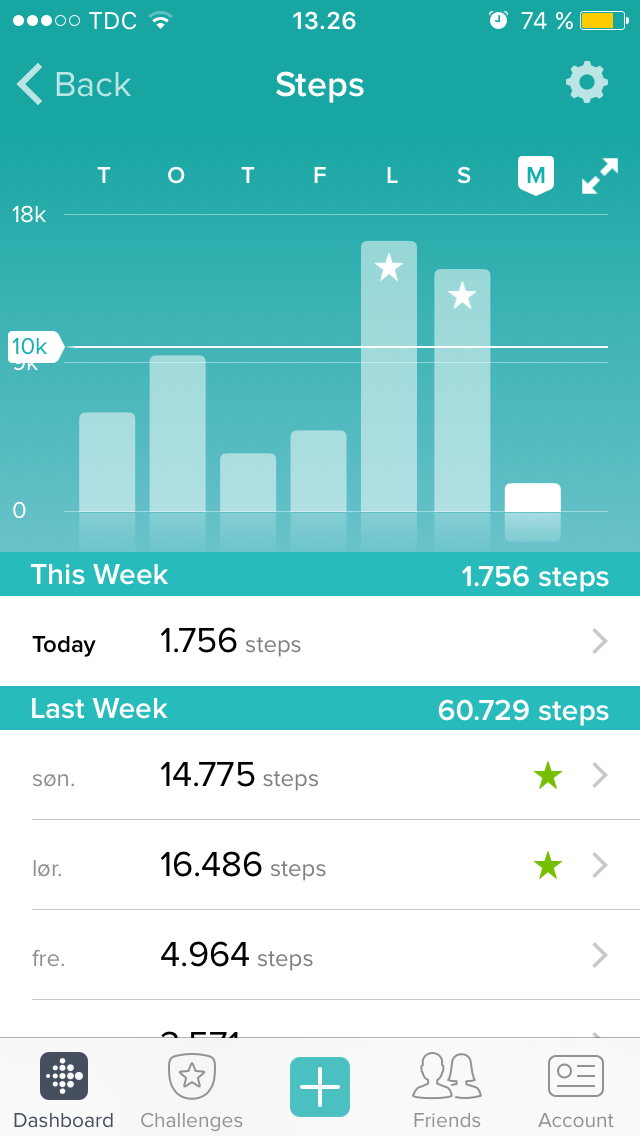
\includegraphics[width=0.45\textwidth]{figures/brugerfladesteps}
	\caption{Oversigt over skridt taget for forhenværende dage, som graf (øverst) og tabel (nederst).}
	\label{fig:brugerfladesteps}
\end{figure}

Af \autoref{fig:brugerfladesteps} ses der foroven en graf over skridt taget inden for den sidste uge. Af grafen ses en hvid tværgående linje, der repræsenterer målet for antal skridt for dagen. Hertil ses at dage hvor målet er blevet opfyldt markeres med en stjerne.  

Under grafen ses en oversigt over antal skridt taget for de forhenværende dage, rækkende tilbage til den første anvendelsesdato. Heraf ses ligeledes at dagene hvor målet nåes, er indikeret med en stjerne. 

Ved at trykke på en den givne dag eller en af de forhenværende dage, kan der ses en mere detaljeret oversigt over skridt taget i løbet af den pågældende dag. Dette ses af \autoref{fig:specifiksteps}, hvor det er muligt at se på hvilke tider af dagen brugeren er mest aktiv.  

\begin{figure}[H]
	\centering
	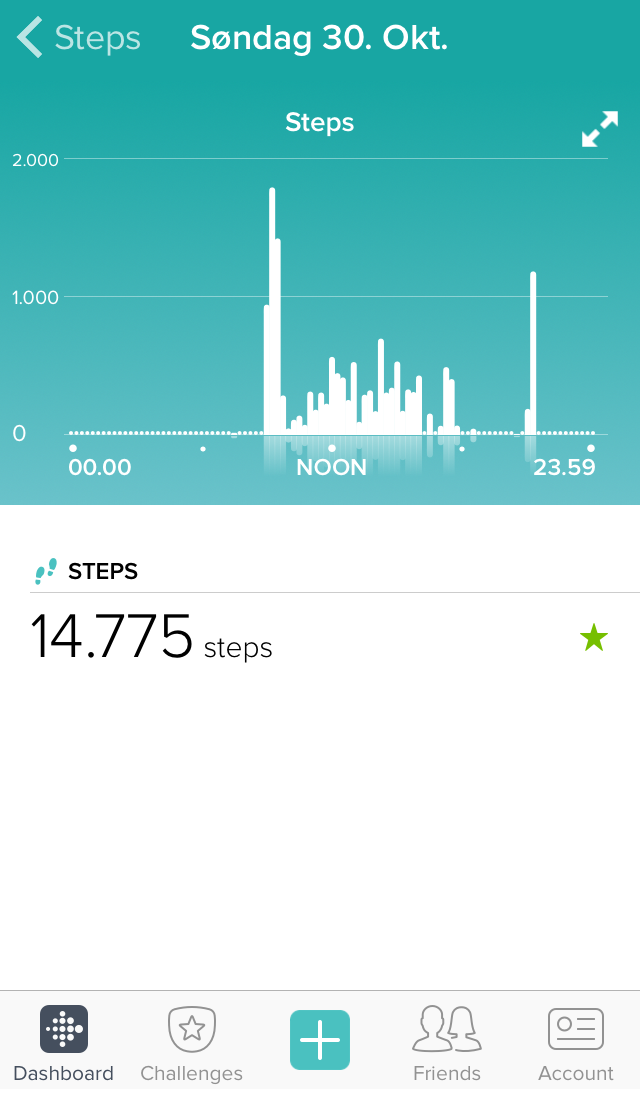
\includegraphics[width=0.45\textwidth]{figures/specifiksteps}
	\caption{Til venstre ses den grafiske oversigt over antal skridt taget, og højre figur viser skridt taget i en tabel.}
	\label{fig:specifiksteps}
\end{figure}


\subsection{Brugertilpasning}
Der er forskellige muligheder for at tilpasse armbåndet optimalt til den givne bruger. Heriblandt er der mulighed og at udskifte armbåndet til andre længder, og at tilpasse skridtlængden til den enkelte bruger. Foruden dette tilegner armbåndet sig og at bliver brugt under forskellige vejrforhold, da Fitbit Flex er vandafvisende. 

\subsubsection{Forskellige størrelser armbånd}
For brugeren er der mulighed for at vælge mellem to forskellige længder af armbånd. Dette tillader muligheden for bedre tilpasning omkring håndleddet. Armbåndene kan ligeledes fås i forskellige farver. % Swag 

\subsubsection{Kalibrering}
Som standard vurderer applikationen brugerens skridtlængde, ud fra de angivne oplysninger ved oprettelsen af brugerkontoen. Brugeren har dog mulighed for at kalibrerer denne værdi, i tilfælde af at brugeren opdager uoverensstemmelse mellem registrerede værdier og reelle værdier. Brugeren kan under indstillinger i applikationen ændre den pre-defineret skridtlængde, til en mere passende. Fitbit oplyser på deres support-hjemmeside guidelines for hvordan brugeren selv udregner værdier til en mere passende skridtlængde.   

\begin{comment}
Hvad består teknologien af?
Hvor udbredt er teknologien?
Hvordan tilpasses teknologien den enkelte person?
Levetid for teknologien?
Hvilke muligheder er der for lagring og videregivelse af information til en læge?
\end{comment}
